\documentclass[11pt]{jarticle}

\usepackage[dvipdfmx]{graphicx}

\setlength{\oddsidemargin}{-6.35mm}
\setlength{\textwidth}{171.9mm}

\begin{document}

\title{画像処理実験 第3回}
\author{09430509\\今田将也}
\date{2020年10月8日}
\maketitle

\section{1.jpg を 0.jpg に重ねる3x3行列m10の計算法の詳細の手順の確認}
初期状態が以下の表を確認する.この動作は行列 $A^{T}$($Q^{T}$), R, ベクトル $b^{T}$, $tmp^{T}$という操作で,
45回実行することで,4組の対応点の座標から射影変換行列が計算される.

\tiny
\begin{verbatim}
    initialized
     256.000000        0.000000      347.000000        0.000000      263.000000        0.000000      413.000000        0.000000 
     218.000000        0.000000      220.000000        0.000000      367.000000        0.000000      315.000000        0.000000 
       1.000000        0.000000        1.000000        0.000000        1.000000        0.000000        1.000000        0.000000 
       0.000000      256.000000        0.000000      347.000000        0.000000      263.000000        0.000000      413.000000 
       0.000000      218.000000        0.000000      220.000000        0.000000      367.000000        0.000000      315.000000 
       0.000000        1.000000        0.000000        1.000000        0.000000        1.000000        0.000000        1.000000 
  -94976.000000   -58880.000000  -160661.000000   -79810.000000  -100729.000000   -99677.000000  -218890.000000  -135051.000000 
  -80878.000000   -50140.000000  -101860.000000   -50600.000000  -140561.000000  -139093.000000  -166950.000000  -103005.000000 

       0.000000        0.000000        0.000000        0.000000        0.000000        0.000000        0.000000        0.000000 
       0.000000        0.000000        0.000000        0.000000        0.000000        0.000000        0.000000        0.000000 
       0.000000        0.000000        0.000000        0.000000        0.000000        0.000000        0.000000        0.000000 
       0.000000        0.000000        0.000000        0.000000        0.000000        0.000000        0.000000        0.000000 
       0.000000        0.000000        0.000000        0.000000        0.000000        0.000000        0.000000        0.000000 
       0.000000        0.000000        0.000000        0.000000        0.000000        0.000000        0.000000        0.000000 
       0.000000        0.000000        0.000000        0.000000        0.000000        0.000000        0.000000        0.000000 
       0.000000        0.000000        0.000000        0.000000        0.000000        0.000000        0.000000        0.000000 

     371.000000      230.000000      463.000000      230.000000      383.000000      379.000000      530.000000      327.000000 

       0.000000        0.000000        0.000000        0.000000        0.000000        0.000000        0.000000        0.000000 
\end{verbatim}
\normalsize

45回実行後の行列が以下のようであった.
\tiny
\begin{verbatim}
    done
       0.392371        0.000000        0.531847        0.000000        0.403100        0.000000        0.633005        0.000000 
       0.013540        0.000000       -0.437106        0.000000        0.876890        0.000000       -0.199546        0.000000 
       0.746709        0.000000        0.224407        0.000000       -0.041838        0.000000       -0.624754        0.000000 
       0.000000        0.392371        0.000000        0.531847        0.000000        0.403100        0.000000        0.633005 
       0.000000        0.013540        0.000000       -0.437106        0.000000        0.876890        0.000000       -0.199546 
       0.000000        0.746709        0.000000        0.224407        0.000000       -0.041838        0.000000       -0.624754 
      -0.295032       -0.448602        0.378993        0.576267        0.142043        0.215980       -0.226004       -0.343644 
      -0.448602        0.295032        0.576267       -0.378993        0.215980       -0.142043       -0.343644        0.226004 

     652.443867      549.877189        1.960322        0.000000        0.000000        0.000000  -301875.042231  -248248.300143 
       0.000000      165.750042        0.253778        0.000000        0.000000        0.000000    24290.303105   -46513.794686 
       0.000000        0.000000        0.304524        0.000000        0.000000        0.000000    33993.758735    26933.037130 
       0.000000        0.000000        0.000000      652.443867      549.877189        1.960322  -191217.160969  -167855.917552 
       0.000000        0.000000        0.000000        0.000000      165.750042        0.253778   -26368.674762   -79976.364619 
       0.000000        0.000000        0.000000        0.000000        0.000000        0.304524    26667.777043    21377.198091 
       0.000000        0.000000        0.000000        0.000000        0.000000        0.000000     7596.900540     1712.683064 
       0.000000        0.000000        0.000000        0.000000        0.000000        0.000000        0.000000     5458.391125 

     371.000000      230.000000      463.000000      230.000000      383.000000      379.000000      530.000000      327.000000 

       0.980063        0.155844       98.500361       -0.055756        1.153389        0.503900       -0.000139        0.000316 
\end{verbatim}
\normalsize

\section{C言語による実装例}
講義ページ内のC言語による実装のファイルを編集した.具体的には,MatrixQRDecompColMajor関数と
MatrixSimeqLr関数を書き換えた.この2つの関数には,8行8列分の操作はなかったため,すでに記載してある手続きと,
資料のPDFの4組の愛横転の場合の射影変換行列を参考に実装をした.

まず,MatrixQRDecompColMajorは,資料のPDF内の式(12)からの処理を行う. 
なお,実装例の配列aTが3行分しか用意されいていないが,実際には8行分必要であることに注意して,
以下のように8行分宣言を行った.
\begin{verbatim}
  double *aT[] = {  Row(mt,0), Row(mt,1), Row(mt,2), Row(mt,3), Row(mt,4), 
                    Row(mt,5), Row(mt,6), Row(mt,7) } ;
\end{verbatim}
次のようなAの各列を$a_{i}$と表した行列
\begin{equation}
  A \colon = [a_{0}, a_{1}...], R \colon = (r_{ij})
\end{equation}


行列は,資料のPDFの式(12)から式(21)によりQに書き換えられ,積QRはもとのAと等しくなる.
具体的な動作手順としては,$a_0$の場合,単位ベクトルへの変換.$a_1$の場合,1回の直交化と単位ベクトルの変換.
$a_2$の場合,2回の直交化のための動作と単位ベクトルへの変換というように規則に沿ったものになっている.
なお,この過程で,Rの要素も得られており,式 (12), 式 (14), 式 (17) 等の分母が対角項$r_{ii}$,式 (13),
式 (15), 式 (16) 等の内積 ($a^{T}_{i}$ $a_j$ ) が非対角項 $r_{ij}$ である.
その実装のソースを一部抜粋したのを以下で示す.

\begin{verbatim}
   Elem(mtR,0,0) = t = sqrt(VP(aT[0],aT[0],W));
   VSS(aT[0], 1/t, W);

 ///////////
   Elem(mtR,0,1) = t = VP(aT[0], aT[1], W);
   VSA(aT[1], aT[0], -t, W);

   Elem(mtR,1,1) = t = sqrt(VP(aT[1],aT[1],W));
   VSS(aT[1], 1/t, W);

 ///////////
   Elem(mtR,0,2) = t = VP(aT[0], aT[2], W);
   VSA(aT[2], aT[0], -t, W);

   Elem(mtR,1,2) = t = VP(aT[1], aT[2], W);
   VSA(aT[2], aT[1], -t, W);

   Elem(mtR,2,2) = t = sqrt(VP(aT[2],aT[2],W));
   VSS(aT[2], 1/t, W);
\end{verbatim}

次に,MatrixSimeqLrはPDF内の式(22)の後ろに書いてある後退代入を行う.
上三角行列で有ることに注意する.
\begin{eqnarray}
  x_2 = t_2 / r_{22}\\
  x_1 = (t_1 - x_2 r_12)/r_{11}\\
  x_0 = (t_0 - \sum_{i=1}^{2} x_i r_{0i})/r_{00}
\end{eqnarray}
目的の解がi個なら,$x_{i}$のiが小さくなるにつれ,引いていく要素が多くなる.
3x3の例を参考に,8x8の実装したもののソースコードの一部を抜粋したものを示す.

\begin{verbatim}
  B[7] =  B[7] / Elem(mtR,7,7);
  B[6] = (B[6]-B[7]*Elem(mtR,6,7)) / Elem(mtR,6,6);
  B[5] = (B[5]-B[6]*Elem(mtR,5,6)-B[7]*Elem(mtR,5,7)) / Elem(mtR,5,5);
  B[4] = (B[4]-B[5]*Elem(mtR,4,5)-B[6]*Elem(mtR,4,6)-B[7]*Elem(mtR,4,7)) / Elem(mtR,4,4);
\end{verbatim}

これを実装し,実際に出力された画像を図\ref{syuturyoku}に示す.

\begin{figure}[ht]
  \centering
  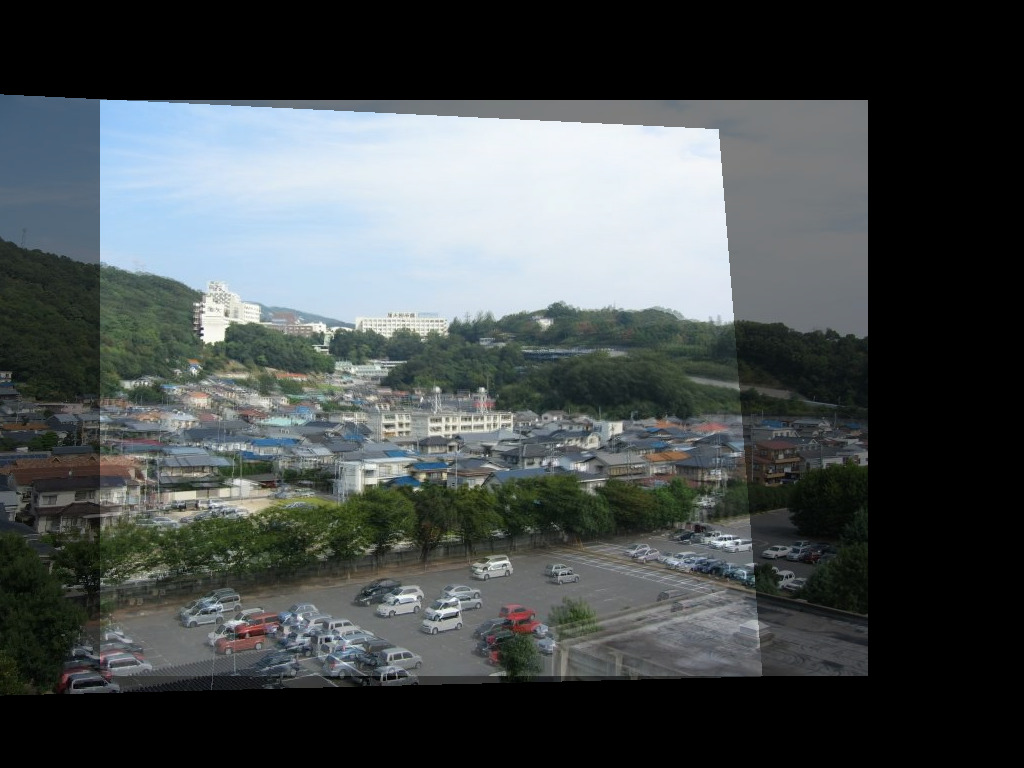
\includegraphics[scale=.2]{syuturyoku.jpg}
  \caption{実際に出力された画像}
  \label{syuturyoku}
\end{figure}

\section{どのような大きさの行列でも扱えるように,ループを用いて実装}

まず,MatrixQRDecompColMajorの配列の個数を動的に確保することから始めた.
\begin{verbatim}
  double **aT = (double **)malloc((sizeof (double *)) * mt->H);
\end{verbatim}
配列の確保はmallocでポインタのポインタaTと宣言することで,後の処理で配列のように扱える.
double **aTという宣言は,ポインタaTが示す先もポインタ*aTであり,そのポインタ*aTという宣言は,ポインタaTが示す先もポインタ
**aTであるということである.
その状態で,mallocにより,double *ポインタを目的の要素分宣言することで,配列要素aT[mt->H]分
求めることができる.この配列aT[0],aT[1]...はポインタであり,その示す先の*at[0],*aT[1]...は
double型であり,ポインタの配列を宣言することになる.その後,aT[0]からaT[mt->H]までの
各要素にRowを格納することでmt->Hがいくらであっても確保できる.

\begin{verbatim}
  double **aT = (double **)malloc((sizeof (double *)) * mt->H);
  //縦に伸びていく 
  for(int get=0; get<mt->H;get++){
      aT[get] = Row(mt,get);
  }
\end{verbatim}


そして,その後のシュミットの直交化手順だが,二重ループを用いた.
確保した要素分(W個分)のaT[i]について手続きを施す.iが増えるに連れ,行うVSA(ベクトルのスカラ倍加算)の回数も増えることに
注意すると,その回数はiを超えない回数行う事となる.
そして,jとiが同じ時にベクトルを単位ベクトルにする動作をする.

以下がそのソースコードである.
\begin{verbatim}
  for(int i=0; i < W; i++){
    for(int j=0; j <= i; j++){
        // printf("%d,%d\n",i,j);
        if(j == i){
            Elem(mtR,j,i) = t = sqrt(VP(aT[j],aT[i],W));
            VSS(aT[i], 1/t, W);
        }else{
            Elem(mtR,j,i) = t = VP(aT[j], aT[i], W);
            VSA(aT[i], aT[j], -t, W);
        }
    }
}
\end{verbatim}

もう一つ,MatrixSimeqLrについて.要素数は,mtR->Wにより可変的に行うことができる.
ここで,8x8の場合を考えてみる.配列の要素数は0~7の8個である.
B[7]の場合,自身をElem(mtR,7,7)で割る動作のみ,B[6]の場合,自身からB[7]にElem(mtR,6,7)をかけたものを引き,Elem(mtR,6,6)で割る.
B[5]の場合,自身からB[6]にElem(mtR,5,6)をかけたものを引き,B[7]にElem(mtR,5,7)をかけたものを引き,Elem(mtR,6,6)で割るという手続きが続く.
これを2重ループに落とし込むと,大きいループの回数は,要素数個分繰り返す.今回は,iの大きい順から手続きを施した.
一度初回を飛ばし,2回目のループであるi=6のときについて考えると,i+1 = 7で一つ大きい添字の要素を参照でき,$\sum$ と同等の処理を内部のループで行える.
$\sum$のくりかえし最大回数は,要素数個分であるから,mtR-\verb|>|W = 8 つまり,配列の添字7までである.
その後,Elemで割るという動作を行えば良い.
では初回のi=7の時を見てみる.一つ添字の大きい要素は8だが,内部の$\sum$にあたるループの上限7を超えているのでループは実行されず,
自身をElemで割るという動作のみ行われることになる.

以下そのソースコードである.
\begin{verbatim}
  for(int i=mtR->W-1; 0<=i; i--){
    for(int j=i+1; j<mtR->W; j++){
      B[i] -=  B[j]*Elem(mtR,i,j);
    }
    B[i] = B[i] / Elem(mtR,i,i);
  }
\end{verbatim}

実行したところ,図\ref{syuturyoku}と同じ結果が得られた.

\section{合成画像の品質を改善}
元々示されていた特徴点は,
\begin{verbatim}
  256,218,  371,230,
  347,220,  463,230,
  263,367,  383,379,
  413,315,  530,327,
\end{verbatim}
だが,出力された画像は図\ref{syuturyoku}であり,あまり精度がよくない.
それを以下のように変更し,なるべく特徴点同士が離れるようにした.
\begin{verbatim}
  147,535,268,544,
  116,209,235,224,
  509,205,629,210,
  432,517,550,530
\end{verbatim}

それにより実行した結果が図\ref{kaizen}である.少し粗はあるものの,図\ref{syuturyoku}と比べると大きく改善しただろう.
\begin{figure}[ht]
\centering
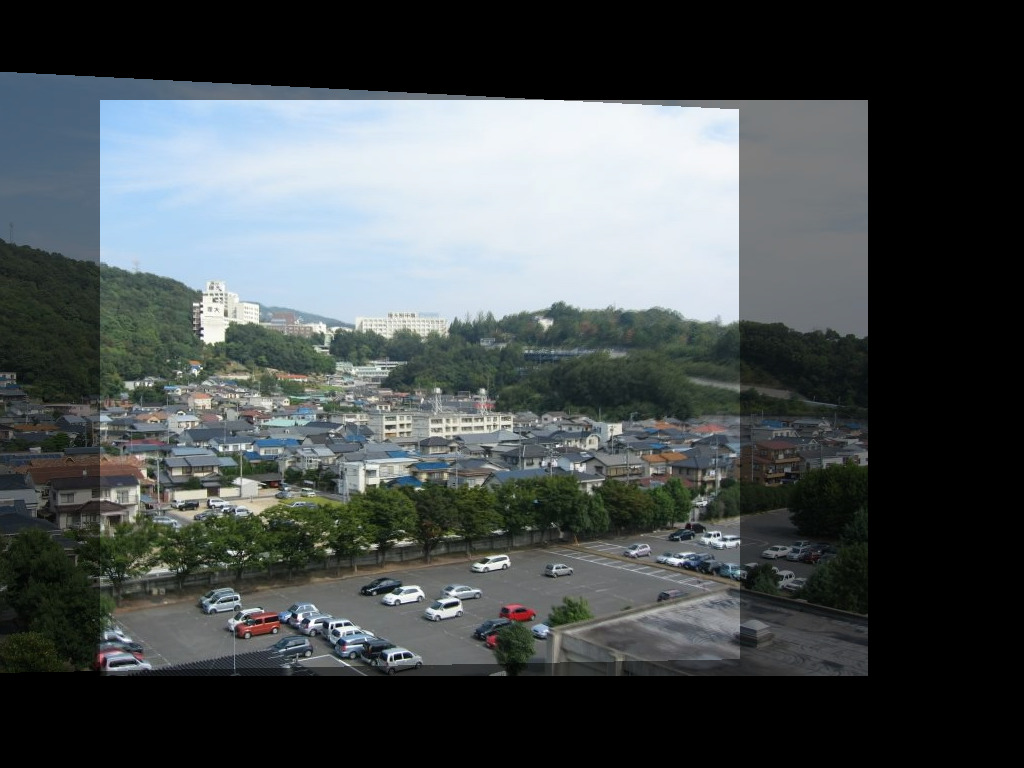
\includegraphics[scale=.3]{kaizen.jpg}
\caption{特徴点の改善後}
\label{kaizen}
\end{figure}

\section{自分で撮影した画像を合成}
撮影した画像がとても大きいサイズだったため,実験同様768x576までサイズを落として実行した.
合成に用いた画像は,図\ref{itimaime},図\ref{nimaime}である.
正確に同じ視点を撮ることができなかったため,真横に100px分だけ移動した画像になっている
特徴点は,以下のように設定した.
\begin{verbatim}
  215,320,  315,319,
  220,507,  320,506,
  651,480,  751,479,
  600,135,  700,134
\end{verbatim}

\begin{figure}[ht]
  \begin{minipage}{0.5\hsize}
    \centering
    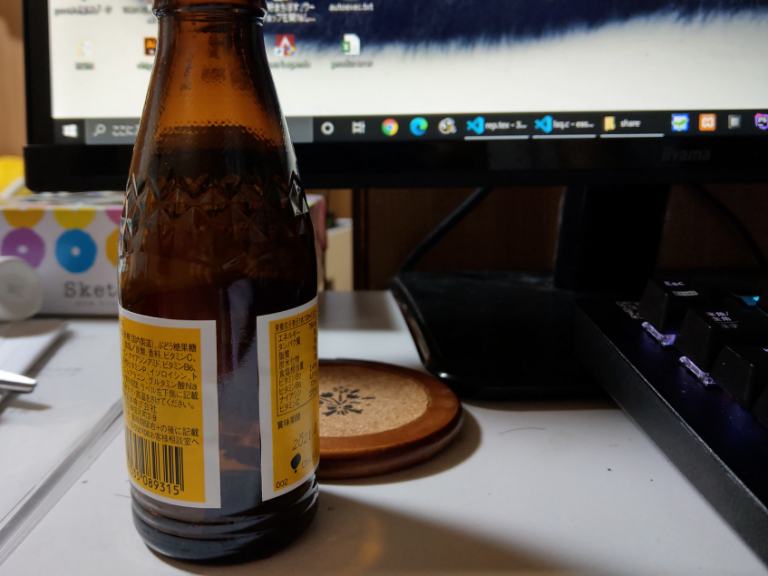
\includegraphics[scale=.3]{mae.jpg}
    \caption{合成1枚目}
    \label{itimaime}
  \end{minipage}
  \begin{minipage}{0.5\hsize}
    \centering
    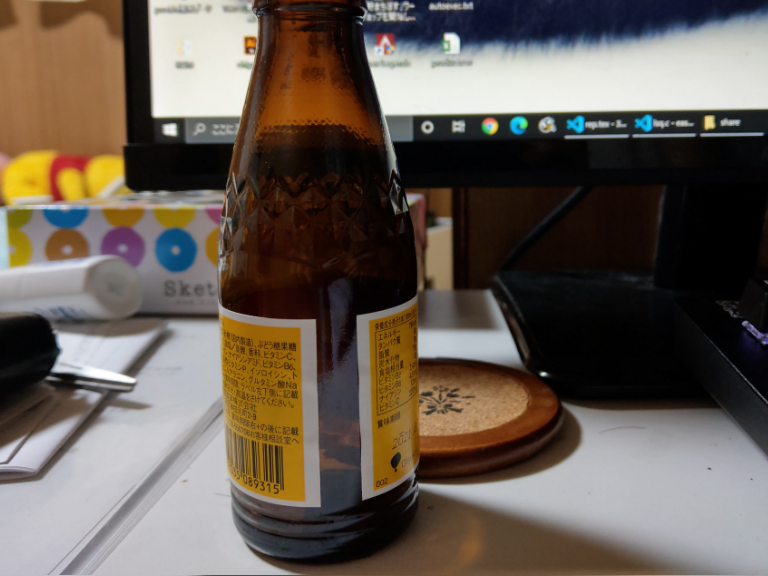
\includegraphics[scale=.3]{ato.jpg}
    \caption{合成2枚目}
    \label{nimaime}
  \end{minipage}
\end{figure}

プログラムを実行すると,図\ref{jibun}のようなパノラマ画像が合成された.
\begin{figure}[t]
  \centering
    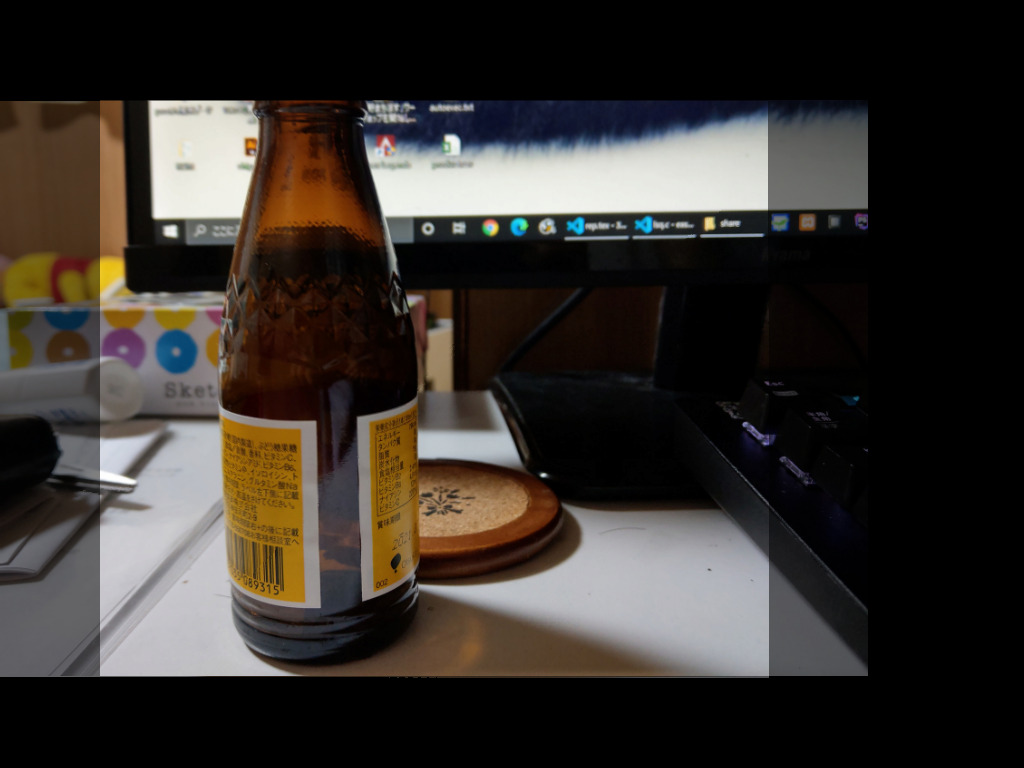
\includegraphics[scale=.5]{jibun.jpg}
    \caption{自分で撮影した画像のパノラマ}
    \label{jibun}
  \end{figure}
\section{感想}
シュミットの直交化をループを使い動的に配列も確保し,8個以上に対応させる箇所について,
for文を回す条件の指定が難航し時間がかかったが,なんとか実装することができた.for文よりも
dowhile文で条件を指定したほうが,わかりやすいプログラムになるとも思ったので,改善事項にしたい.

また,自分で撮影した画像のパノラマの,同じ視点というものに苦労した.最終的に一枚の画像を切り抜き,
横に移動させたもので同一の視点ということにしたが,実際にそんな画像を人間の手で道具なしで撮るのは難しいため,
スマホに搭載されているパノラマの機能は高度だと感じた.しかし,自分が撮った画像のパノラマがCにより書き出された時は
感動した.

なお,4個以上の特徴点を用いた実装や,3枚以上の画像の合成は取り組めなかったため,今後の課題としたい.
\end{document}
